\subsection*{Motivation}
%--------------------------------------------------------------------------------------------------
\begin{frame}[t]
    \frametitle{Interpretable Gradients}
    \framesubtitle{Leveraging Backpropagation}
    \small 
    The response ($y$) of a model ($f$) parameters ($\phi$) , after forwarding an input $x$ can be 
    visualized on the input space, via backpropagation:
    \begin{equation}
        \frac{\partial x}{\partial y} = \frac{\partial x}{\partial F_0}\frac{\partial F_0}{\partial F_1}\cdot\dots\cdot\frac
        {\partial F_{-1}}{\partial y}
        \label{eq:backtoin}
    \end{equation}
    \pause
    However, due to non-linearities it is noisy:
    \begin{columns}
        \column{.2\textwidth}
        \column{.3\textwidth}
            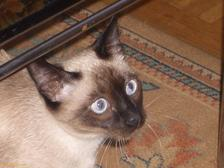
\includegraphics[width=.95\textwidth]{fig/gradient/fig/Original_Input.JPEG}
        \column{.3\textwidth}
            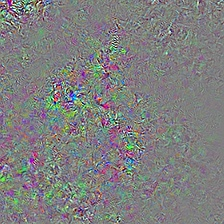
\includegraphics[width=.95\textwidth]{fig/gradient/fig/method/gradient.jpg}
        \column{.2\textwidth}
    \end{columns}
\end{frame}
%--------------------------------------------------------------------------------------------------
\begin{frame}[t]
    \frametitle{Interpretable Gradients}
    \framesubtitle{Soft Gradients}
    \small
    Soft gradients can be achieved by two approaches:
    \begin{columns}
        \footnotesize
        \column[T]{.5\textwidth}
            \textbf{Guided Backpropagation \cite{guidedbackprop}}\\
            Achieved by constraining backprop to only let 
            positive gradients flow:
            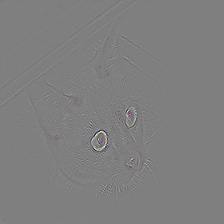
\includegraphics[width=.80\textwidth]{fig/gradient/fig/gb_standard.jpg}
            \pause
        \column[T]{.5\textwidth}
            \textbf{Smoothgrad \cite{smilkov2017smoothgrad}}\\
            Achieved by iteratively adding noise to the input space prior to forward pass:
            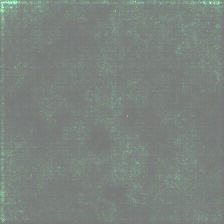
\includegraphics[width=.80\textwidth]{fig/gradient/fig/gb_smooth.jpg}
    \end{columns}
\end{frame}